\documentclass{article}
\usepackage[utf8]{inputenc}
\usepackage[margin=1in]{geometry}
\usepackage{graphicx}
\usepackage{float}
\usepackage[utf8]{inputenc}
\usepackage{caption}
\usepackage{subcaption}
\title{SoftDes Mini Project 3 Write Up}
\author{Sam Coleman}
\date{March 7, 2020}

\begin{document}

\maketitle

\section{Project Overview}
Using the Tweepy wrapper for the Twitter API, I compared and analyzed the word choices of the top two Democratic candidates (Bernie Sanders and Joe Biden) and President Trump from their tweets. After pulling the tweets, the full text of tweets are stored in a pickled file. I created a word frequency dictionary with the words as keys and the corresponding frequencies as the values. I removed words with little meaning such as 'the' and 'of.' The dictionary is then taken and the top \textit{n} words are shown for each candidate. To visualize the data, a word cloud for each candidate is created using the WordCloud library. The function uses the frequency dictionary to display the top words with the size correlating to the frequency used. Through this project, I aimed to implement an API and research other libraries I could use in my programs to expand functionality.  

\section{Implementation}
To make my code clear and organized, it is separated into two files. The first file contains what actually calls the Twitter API (through the Tweepy wrapper) to retrieve recent Tweets from Trump, Bernie, and Biden and does some basic cleaning of the data. The text of the tweets for each user are stored in a list. After they are retrieved, the text is broken up into single words and placed in a new list which is put into a pickle file. To avoid calling the API more than needed, if the file name already exists for a user, the pickled file is loaded in instead of re-running the API. This also significantly speeds up the code as Tweepy takes a long time to pull all the tweets. In the analyze\_tweets document, a dictionary is created with a word as keys and the corresponding frequencies as values. In addition to creating a word cloud from this dictionary for each candidate by utilizing the WordCloud library, there is also a function to write the top \textit{n} words into a text file in order of frequency. This provides an additional way to interpret the data. 
\bigskip
A major design decision I came across was the option between using Twitter API directly or using the Tweepy wrapper. I began by using the Twitter API directly as described on the SoftDes website. In recent years, Twitter updated their API to limit number of Tweets to try and retrieve, up to a maximum of 200 per distinct request. This significantly decreased the sample size of tweets received by my program, and after extensive research, the Tweepy wrapper seemed like the best alternative. The Tweepy Cursor function calls the api.user\_timeline multiple times while iteration through each tweet. This allows the program to gather well over 200 tweets without much extra code.

\section{Results}

The images below are the word clouds for the top 50 words used by Trump, Bernie, and Biden in their tweets. The size of the word corresponds to the frequency it is used.

    
\begin{figure}[H]
    \centering
    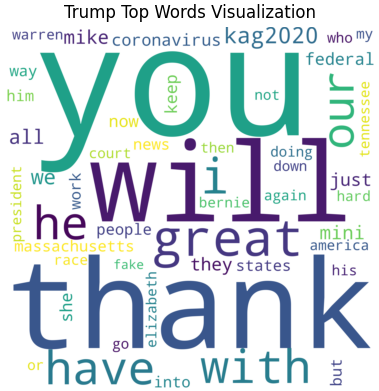
\includegraphics[width=9cm]{TrumpWordCloud50Crop.png}
    \caption{Trump's Top 50 Words Word Cloud}
    \label{fig:trump50}
\end{figure}

\begin{figure}[H]
    \centering
    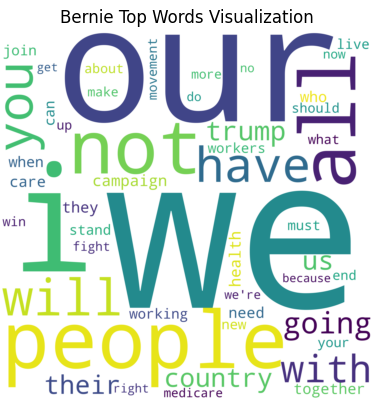
\includegraphics[width=9cm]{BernieWordCloud50Crop.png}
    \caption{Bernie's Top 50 Words Word Cloud}
    \label{fig:bernie50}
\end{figure}

\begin{figure}[H]
    \centering
    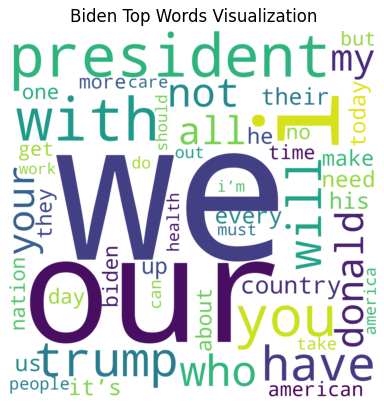
\includegraphics[width=9cm]{BidenWordCloud50Crop.png}
    \caption{Biden's Top 50 Words Word Cloud}
    \label{fig:biden50}
\end{figure}

As figure \ref{fig:trump50} displays, Trump's top two words are "you" and "thank." This is in contrast to figures \ref{fig:bernie50} and \ref{fig:biden50} who both use "we" and "our" the most. This is interesting, as it shows that Trump is trying to relate to the individual. By saying "you," he tries to make a personal connection with the people. Additional, he thanks a lot of people on twitter so "thank you" is a phrase often used. This is very different than both Bernie and Biden who try to bring people together in their tweets. "We" and "our" has the effect of bringing people together. Bernie and Biden are trying to convey that it is a group effort, and that change will not happen with an individual, but rather, all of us coming together.\newline
To understand the word choices even more, below are the top 50 words used by the candidates in order of their frequency. 
\begin{itemize}
    \item \textbf{Trump}: you, thank, will, great, i, with, have, he, our, kag2020, we, all, mini, mike, just, they, coronavirus, now, federal, keep, she, way, news, but, people, states, into, massachusetts, him, work, my, tennessee, doing, court, america, again, then, who, president, not, hard, elizabeth, warren, bernie, or, his, down, go, race, fake
    \item \textbf{Bernie}: we, our, i, people, all, not, will, you, have, with, going, trump, us, country, their, campaign, health, care, they, who, together, need, when, can, join, stand, working, must, new, workers, live, your, end, should, what, about, up, make, win, movement, more, now, do, fight, medicare, we're, no, right, get, because
    \item \textbf{Biden}: we, our, i, president, with, you, trump, have, will, who, not, all, donald, your, my, country, their, his, every, us, up, it's, need, today, he, make, about, they, biden, day, no, one, nation, american, get, more, time, but, people, take, care, can, out, health, do, must, america, should, i'm, work
\end{itemize}

The below word clouds have a maximum of 200 words displayed. While the top 50 words are a good amount to analyze, it is still interesting to visualize more words than this as all three candidates have vastly different word choices. These word clouds include more words than the top 50, and are very interesting to look at and compare. Trump's nicknames for candidates show up for his frequent words, such as "Mini Mike." While both Bernie and Biden mention Trump, they do not use a nickname for him or anyone else.

\begin{figure}[H]
    \centering
    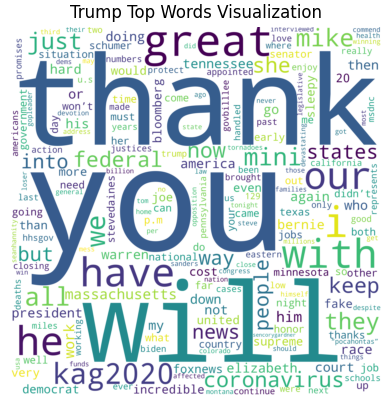
\includegraphics[width=9cm]{TrumpWordCloudCrop.png}
    \caption{Trump's Full Word Cloud}
    \label{fig:trumpFull}
\end{figure}

\begin{figure}[H]
    \centering
    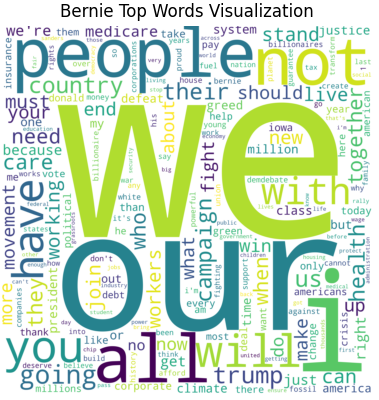
\includegraphics[width=9cm]{BernieWordCloudCrop.png}
    \caption{Bernie's Full Word Cloud}
    \label{fig:bernieFull}
\end{figure}

\begin{figure}[H]
    \centering
    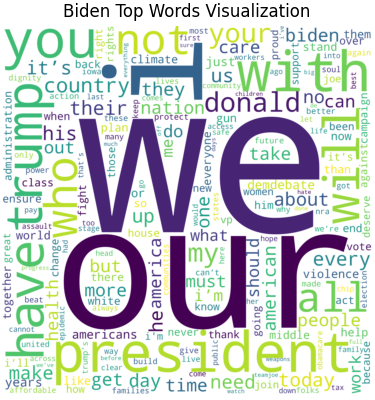
\includegraphics[width=9cm]{BidenWordCloudCrop.png}
    \caption{Biden's Full Word Cloud}
    \label{fig:bidenFull}
\end{figure}

\section{Alignment}
Overall, there is a good amount of alignment between what I set out to explore and the data and tools used to carry out the project. I set out to explore the word choices of Trump, Bernie, and Biden in their tweets. That guiding question sparked my exploration as the primary elections are currently occurring. I was curious to see if Trump's word choices were different than that of the leading Democratic Candidates, and how the tweets of the Democratic Candidates compared. Upon completion, I imagined an answer would look like word clouds for the users. As language has a lot of nuances, I didn't want to compare the lists directly. Words have correlations to other words and ideas, and creating a frequency based word cloud would be an effective way to interpret and understand the information. \\
\bigskip
At the beginning of the project, I thought there would be few limitations because I was gathering the data directly from Twitter using the API. However, as discussed in the Implementation section, there was difficulty in collecting a large sample size of tweets. A larger unanticipated limitation was the difficulty of gathering Trump's tweets. While using the functions in get\_tweets.py worked perfectly for gathering a large number (between 2,000-3,000) of tweets for both Bernie and Biden, it was not consistent for Trump. For Trump, it would get a different number of tweets every time I ran it, ranging from 1-350 tweets. After working on this for many hours, including talking to multiple NINJAs, Amon, and Steve, we determined that Twitter is rate-limiting the pulling of Trump's tweets. My program is using the file with the largest number of Trump tweets pulled (about 350). This adds a level of inaccuracy in the program since the sample size of Trump and the other candidates are significantly different. There is no easy way around this, and I decided to cut my loses and continue the project with just 350 Trump Tweets. The main problem with this is that the Trump tweets I have are rather recent, so current events such as the coronavirus are more heavily displayed as they probably would have been if I was able to get 2,000-3,000 Trump tweets like I did for the other candidates. \\
\bigskip
I think despite the limitations, the answers are rather accurate. Using the Tweepy wrapper helped significantly in increasing the sample size. Using the WordCloud library aided a lot in the visualization of the information. There is a higher level of confidence with Bernie and Biden because of the sample size and range of dates from the tweets. If I were able to acquire more tweets from Trump, the confidence would increase but this is not possible using an API because of Twitter limits. 

\section{Reflection}
Overall, I think this project went well. Although I wish I had started working a little sooner than I did, my schedule has been really full. When I did start, I made a lot of progress in a short amount of time and never felt like I was running out of time. When I was stuck on various API problems, I went to NINJAs hours, which helped me a lot to move forward and make progress. One way I could mitigate the Trump rate limit problem would be to scrape an html page of an archive of his Tweets, or work with a csv archive of his tweets. I want to do this in the future to improve this project, I just did not have enough time during the span of this project. I think my project was appropriately scoped, as I had many ideas of paths I could take if I had more time to work on the project. This includes working to acquire more Trump tweets through html scraping or csv file, using the NLTK, or doing Markov text synthesize. I didn't write any unit tests because I was able to re-use a lot of code I wrote for either reading journals or Toolboxes and I knew they worked. Moving forward, I want to think through the logic flow of my code more before starting. Additionally, I want try to think through what functions I will need sooner in the process. 
\end{document}
